\documentclass[twocolumn,english,notitlepage]{article}
\usepackage[margin=0.5in]{geometry}
\setlength{\parindent}{0pt} % no indents

% Math
\usepackage{amsmath}
\usepackage{physics}
\usepackage{amsfonts} % for mathbb

% Citetations
\usepackage[ backend=bibtex, sorting=none, autocite=plain]{biblatex}
\addbibresource{refs/references}
\usepackage{xcolor}
\usepackage{hyperref}
\hypersetup{
    colorlinks,
    linkcolor={red!50!black},
    citecolor={blue!50!black},
    urlcolor={blue!80!black}}


% Formatting
\usepackage{float}
\usepackage{graphicx}
\graphicspath{ {./figs/} } 

% Misc
\usepackage{appendix}
\usepackage{xfrac} % provides \sfrac

% Commands

\newcommand{\integral}[1]{\ensuremath{\int\!\mathrm{d}#1\,}}
\renewcommand{\d}[2][x]{\ensuremath{\frac{\mathrm{d}#2}{\mathrm{d}#1}}}

\renewcommand{\vec}[1]{\boldsymbol{#1}}
\newcommand{\pclosed}[1]{\left(#1\right)}
\newcommand{\bclosed}[1]{\left[#1\right]}
\newcommand{\cclosed}[1]{\left\{#1\right\}}
\newcommand{\vclosed}[1]{\left|#1\right|}
\renewcommand{\norm}[2][]{\ensuremath{\|#2\|_{#1}}}
\renewcommand{\exp}[1]{e^{#1}}
\newcommand{\exptext}[1]{\operatorname{exp}\pclosed{#1}}
\newcommand{\dimof}[1]{\bigl[#1\bigr]}

\renewcommand{\expval}{\operatorname{\mathbb{E}}}
\renewcommand{\var}{\operatorname{Var}}
\DeclareMathOperator{\eye}{\mathbb{I}}
\DeclareMathOperator{\sgn}{sgn}

\newcommand{\betahat}{\hat{\beta}}
\newcommand{\msub}[2]{\ensuremath{{#1}_\text{#2}}}

\title{Bias-variance tradeoff in simple linear models} % very much working title
\author{Anna Aasen, Carl Martin Fevang, Håkon Kvernmoen}
\date{\today}

\begin{document}

\twocolumn[
    \begin{@twocolumnfalse}
        \maketitle
        \begin{abstract}
            This is the abstract.
        \end{abstract}
    \end{@twocolumnfalse}
]

\section{Introduction}
    In this project, we will introduce some of the most important general properties of machine learning models in the context of linear regression. Specifically the mean squared error (MSE), the bias and the variance of data predictions are essential in evaluating the quality of a statistical model. We look at the phenomena of underfitting and overfitting, and explore them in the context of bias-variance trade-off. The three models we will use explicitly are Ordinary Linear Regression (OLS), Ridge regression and Least-Absolute-Shrinkage-and-Selection-Operation (LASSO) regression. These will first be tested on the 2D Franke function, and later on real geographical terrain data.

    The aforementioned models will be explored using resampling techniques, which will be employed to extract the relevant statistical quantities in an accurate way. We will use the standard methods of Bootstrapping and Cross Validation and compare the results we get between them across the three linear models.

    All the models will be applied by fitting a two-dimensional polynomial expansion to the observed data.



\begin{figure}[H]\label{fig:intro:plat}
    \centering
    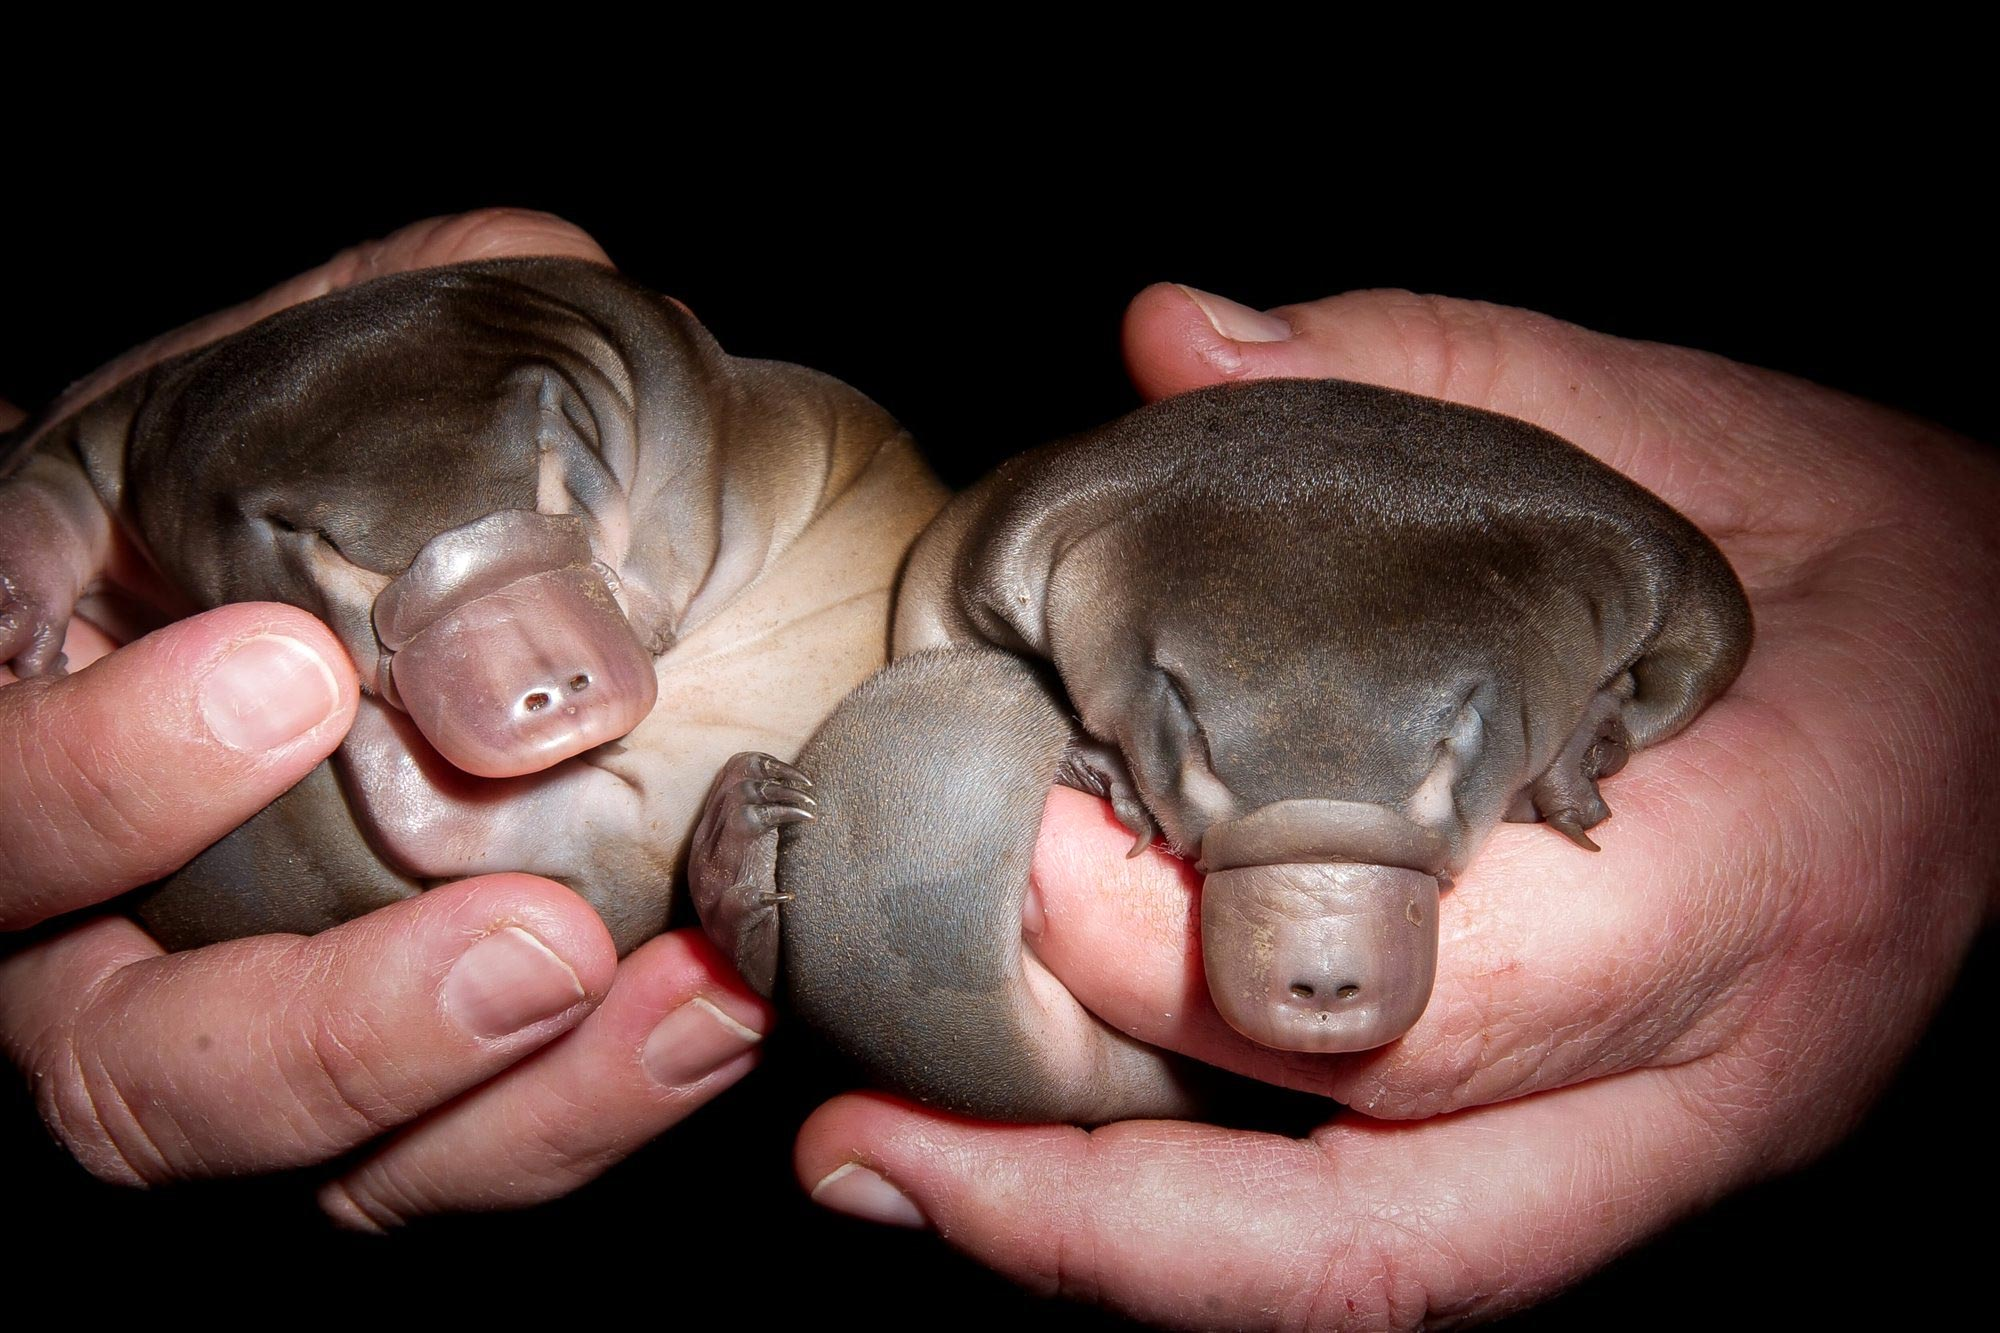
\includegraphics[width=0.5\linewidth]{Young-Platypus.jpg}
    \caption{Some figure caption}
\end{figure}

\section{Theory}
    \subsection{Statistical introduction to linear regression}
        A way to motivate the process of statistical learning is that we want to develop a process by which we use observed data to inform our belief in a future outcome. Such a process can be developed from the ideas of Bayes' theorem, which we can use to inform us what confidence we should have in the parameters of a given model, given data points we have observed.
        
        Let $\vec{y}$ denote a vector of a series of measured values $y_i$, $i\in 1, 2,..., n$ at points $X$, where $X$ is a matrix where the rows $x_i$ correspond to the input values for the measurement $y_i$. For completeness we refer to the columns of $X$ as $\vec{x}_a$, $a=1, 2,..., p$.\footnote{Throughout this project, $a, b$ will always index the $p$ features for a model, and $i, j$ the $n$ data points.} Further let $\vec{\theta}$ denote the parameters of our given model -- then Bayes' theorem tells us that our \textit{posteriori} confidence in the parameters $\vec{\theta}$ given the available data follows
        \begin{align}
            P(\vec{\theta}|X, \vec{y}) = \frac{P(\vec{y}|X,\vec{\vec{\theta}})P(\vec{\theta})}{P(X,\vec{y})}.
        \end{align}
        Here $P(X,\vec{y})$ plays the role of a normalisation, and can safely be ignored -- either because we look for values of $\vec{\theta}$ that maximise the probability, or because we assume the probabilities $P(\vec{y}|X,\vec{\theta})$ and $P(\vec{\theta})$ which we then can properly normalise. Now we have a framework through which we can use assumptions about the distributions $P(\vec{y}|X,\vec{\theta})$ and $P(\vec{\theta})$ to give us a probability distribution for the parameters $\vec{\theta}$ that we can maximise.

        \subsubsection{Ordinary least squares}
            Now we can define the ordinary least squares method by assuming that the data $y$ that we want to make a fit to has a linear noise term that is normally distributed with mean nought. That is, the data is generated as $y(x) = f(x) + \epsilon$, where $f(x)$ is some analytic, non-stochastic function of the data input $x$, and $\epsilon \sim N(0, \sigma^2)$. Further, if we make a model fitting $y(x)$ by a $\tilde{y}(x)$, we should expect the error at every data point $(y_i, x_i)$ to be be normally distributed with the same variance, i.e., independently and identically distributed (i.i.d.). This can be summarised
            \begin{align}
                P(\vec{y}|X, \vec{\theta}) = \prod_{i=1}^{n} \frac{1}{\sqrt{2\pi\sigma^2}} \exp{-\frac{{(y_i-\tilde{y}_i)}^2}{2\sigma^2}}.
            \end{align}
            Furthermore, we assume the parameters $\vec{\theta}$ to be distributed evenly, and as such, $P(\vec{\theta})$ just contributed to an overall normalisation. This means that maximising $P(\vec{y}|X, \vec{\beta})$ amounts to the same as maximising $P(\vec{\theta}|X, \vec{y})$, and can be done analytically.

            Knowing that the Gaussian distribution has a single extremum that is a maximum, we can find the values for $\vec{\theta}$ maximising the probability as
            \begin{align} \nonumber
                \d[\theta_k]{P(\vec{y}|X,\vec{\theta})} &= 0 \\
                \Rightarrow \prod_{i=1}^{n} \frac{1}{\sqrt{2\pi\sigma^2}} \frac{1}{\sigma^2} X_{ib}(y_i-X_{ia}\theta_a) \exp{-\frac{{(y_i - X_{ia}\theta_a)}^2}{2\sigma^2}} &= 0,
            \end{align}
            which as we can see, is maximisable point by point. This means that the optimal parameters $\msub{\vec{\hat{\theta}}}{OLS}$ that maximise $P(\vec{y}|X, \vec{\theta})$ can be found as
            \begin{align}
                \boxed{
                \msub{\vec{\hat{\theta}}}{OLS} = \pclosed{X^TX}^{-1} X^T \vec{y}.
                }
            \end{align}


        \subsection{Ridge and LASSO regression}
            So far, we have assumed that the parameters $\vec{\theta}$ are uniformly distributed, and as such have no \textit{bias} towards any particular value. In practice, this means that the OLS model will contort to fit itself to all values in the data. As such, a motivation for adding a bias could be for the sake of stability in the fit. This is done in ridge regression, where one assumes that the parameters are normally distributed, such that parameter values far from the mean are thought less likely to occurr. This in practice means that the model is less willing to contort to outliers in the dataset, trading it for a bias towards certain parameter values. Assuming the probability distrbution for $\vec{\theta}$
            \begin{align}
                P(\vec{\theta}) = \prod_{a=1}^{p} \frac{1}{\sqrt{2\pi\tau^2}} \exp{-\frac{\theta_a^2}{2\tau^2}},
            \end{align}
            with a derivative with respect to $\theta_b$
            \begin{align}
                \d[\theta_b]{P(\vec{\theta})} = -\prod_{a=1}^{p} \frac{1}{\sqrt{2\pi\tau^2}} \frac{1}{\tau^2} \theta_b \exp{-\frac{\theta_a^2}{2\tau^2}} = -\frac{1}{\tau^2} \theta_b P(\vec{\theta}),
            \end{align}
            the condition for maximising $P(\vec{\theta}|X, \vec{y})$ becomes
            \begin{align} \nonumber
                \d[\vec{\theta}]{P(\vec{y}|X, \vec{\theta})} P(\vec{\theta}) + P(\vec{y}|X, \vec{\theta}) \d[\vec{\theta}]{P(\vec{\theta})} &= 0 \\
                \pclosed{ \frac{1}{\sigma^2} X^T(\vec{y}-X\vec{\theta}) - \frac{1}{\tau^2} \vec{\theta} } P(\vec{y}|X,\vec{\theta}) P(\vec{\theta}) &= 0.
            \end{align}
            Rewriting with a parameter $\lambda = \sigma^2/\tau^2$, the optimal parameters $\msub{\vec{\hat{\theta}}}{ridge}$ are given by
            \begin{align}
                \boxed{
                \msub{\vec{\hat{\theta}}}{ridge} = \pclosed{X^TX + \lambda \eye}^{-1} X^T \vec{y}.
                }
            \end{align}
            This has the added bonus of ensuring that $X^TX + \lambda \eye$ is always invertible, as $\det(\lambda \eye) \neq 0$ for $\lambda>0$.

            LASSO regression builds on the same ideas as ridge regression, by assumes rather a Laplace distribution $L(0, \tau)$ for the parameters $\vec{\theta}$. This gives
            \begin{align}
                P(\vec{\theta}) = \prod_{a=1}^{p} \frac{1}{2\tau} \exp{-\frac{|\theta_a|}{\tau}},
            \end{align}
            which as we can see is not differentiable at $\theta_i = 0$. This means that the optimisation of this the probability $P(\vec{\theta}|X, \vec{y})$ is not necessarily possible analytically without putting bounds on the data $X, \vec{y}$, and even numerical algorithms like gradient descent will encounter run into trouble. Furthermore, it is not optimisable point by point, unless bounds like $X^TX$ being diagonal are enforced, which makes LASSO generally less used. Nevertheless, we can coax a cost function out of the probability that is minimalisable. Letting the cost function be written $\msub{C}{lasso}(\vec{\theta}) = -A\log\pclosed{P(\vec{\theta|X,\vec{y}})} + B$  we can choose the constants $A, B$ such that
            \begin{align}
                \boxed{
                    \msub{C}{lasso}(\vec{\vec{\theta}}) = \norm[2]{ \vec{y} - X\vec{\theta} }^2 + \lambda \norm[1]{\vec{\theta}},
                }
            \end{align}
            where $\lambda = \frac{2\sigma^2}{\tau}$ and $\norm[p]{\vec{v}} = \pclosed{\sum_k |v_k|^p}^{\sfrac{1}{p}}$ denotes the $L_p$ norm of the vector $\vec{v} \in \mathbb{R}^k$.

\section{Method}
Something general about initially fitting Franke data using OLS, ridge and lasso. Then moving on to real terrain data something something.
    
    \subsection{Franke function}

    For the initial testing of our implemented fitting routines, we will use the so called \textit{Franke function}. Being able to control the number of sample points and noise levels will serve as a good examination of our models advantages and disadvantaged. Defined for $x, y \in [0,1]$

    \begin{align}
        F(x,y) = f_1(x,y) + f_2(x,y) + f_3(x,y) + f_4(x,y) + \epsilon \label{eq:met:Franke_Function}
    \end{align}

    Where the $f_i(x,y)$ are Gaussian functions, constructed to mimic the shape of a hill top landscape. More concretely, these are defined as:

    \begin{align} \nonumber
        f_1(x,y) &= \frac{3}{4}\exptext{ -\frac{(9x-2)^2}{4} - \frac{(9y-2)^2}{4} } \nonumber \\
        f_2(x,y) &= \frac{3}{4}\exptext{ -\frac{(9x+1)^2}{49} - \frac{(9y+1)}{10}} \nonumber \\
        f_3(x,y) &= \frac{1}{2}\exptext{ -\frac{(9x-7)^2}{4} - \frac{(9y-3)^2}{4}} \nonumber \\
        f_4(x,y) &= -\frac{3}{4}\exptext{ -(9x-4)^2 - (9y-7)^2} \nonumber
    \end{align}

    And $\epsilon$ is some stochastic noise $\epsilon \sim N(0,\sigma^2)$. By visual inspection, we can fine tune $\sigma$ to create data that looks like noisy digital terrain data.
    
    \subsection{Linear regression}
    % not sure about how we should divide these subsection, but I wanted to write a bit about data scaling
    Before fitting our models to the sampled data, we will scale the data using the $Z$-score normalisation. This scales the inputs $x_i$ and the targets $\vec{y}$ such that they have a mean value of $0$ with a standard deviation $1$. In effect, we rescale
    \begin{subequations}
        \begin{align}
            \vec{y}^\text{scaled} &= \frac{\vec{y}-\bar{y}}{\bar{\sigma}_{\vec{y}}}, \\
            \vec{x}_a^\text{scaled} &= \frac{\vec{x}_a - \bar{x}_a}{\bar{\sigma}_{\vec{x}_a}},
        \end{align}
    \end{subequations}
    where $\bar{z} = \frac{1}{n} \sum_{i=0}^n z_n$ detotes the sample mean of $\vec{z}$ and $\sigma_{\vec{z}}^2 = \frac{1}{n} \sum_{i=0}^n {(z_i-\bar{z})}^2$ denotes the sample std of $\vec{z}$.

    \subsection{Resampling techniques}

        \subsubsection*{Bootstrap}

        \subsubsection*{Cross-validation}

\section{Results}

\section{Discussion}
    \subsection{Data scaling}
        % This should probably be a subsubsection within something else. Just summing up the thoughts we have thrown around regarding the necessity and function of scaling.
        % Please read and see if it makes sense at all!
        The scaling of the inputs and measurments can roughly be divided into two operations, each with their own set consequences. Let us first consider shifting of the measurements $\vec{y}$ and the inputs $\vec{x}_a$ by their respective means. Effectively, this eliminates a degree of freedom from our model $\hat{f}(x)$ as we set it mean value to nought, and leave out any parameter that would govern this. However, if we shift $\vec{y}$ to have a mean of nought as well, this degree of freedom becomes redundant, and we end up effectively reducing the dimensionality of the model by one.

        Considering now the rescaling of $\vec{y}$ and $\vec{x}_a$, these affect the fitting of the model more subtely. Looking at it through the lense of dimensionality know that
        \begin{align}
            \dimof{\theta_a} = \dimof{y} / \dimof{x_a}.
        \end{align}
        From this we can infer that the order of magnitude of a parameter $\theta_a$ is governed by the dimension its corresponding feature $\dimof{x_a}$. This matters in the regularised models where a cost is associated with the norm of the parameters $\norm[p]{\vec{theta}}$, which will be dominated by parameters whose dimension is large. In practice, this means that the fitting will focus more on reducing the magnitude of the parameters whose associated dimension is large, letting the others fluctuate more freely. By making the $x_a$'s dimensionless, the parameters are put on a `level playing field', so to speak. The dimension of $y$ serves to raise or lower the order of magnitude of the all the paramers, and can be adjusted as to avoid numerical truncation errors by avoiding larger floats.


\section{Concluding remarks}





\begin{appendix}
    \section{Theoretical proof of concept of the OLS model}
    \begin{align}
        \expval(y_i) = \expval\bclosed{X_{ij} \vec{\beta}_j + \epsilon_i} = X_{ij}\vec{\beta}_j + \expval(\epsilon) = X_{ij}\vec{\beta}_j
    \end{align}

    \begin{align} \nonumber
        \var(y_i) &= \expval\bclosed{\pclosed{y_i-\expval\pclosed{y_i}}^2} = \expval\bclosed{\pclosed{X_{ij}\vec{\beta}_j + \epsilon_i - X_{ij}\vec{\beta}_j}^2} \\
        &= \expval\pclosed{\epsilon_i^2} = \var\pclosed{\epsilon_i} = \sigma^2
    \end{align}

    \begin{align} \nonumber
        \expval(\vec{\betahat}) &= \expval\pclosed{(X^TX)^{-1}X^T \vec{y}} = \expval\pclosed{(X^TX)^{-1}X^T \bclosed{X\vec{\beta} + \vec{\epsilon}} } \\
        &= \expval\pclosed{\vec{\beta}} + {(X^TX)}^{-1}X^T \expval\pclosed{\vec{\epsilon}} = \vec{\beta}
    \end{align}

    \begin{align} \nonumber
        \var(\vec{\betahat}) &= \expval({\vec{\betahat} \vec{\betahat}^T}) - \expval({\vec{\betahat}}) \expval({\vec{\betahat}^T}) \\ \nonumber
        &= \expval((X^TX)^{-1}X^T \vec{y} \vec{y}^T X (X^TX)^{-1}) - \vec{\beta}\vec{\beta^T} \\ \nonumber
        &= (X^TX)^{-1}X^T \bclosed{X\vec{\beta}\vec{\beta}^TX^T + \sigma^2 \eye}X (X^TX)^{-1} - \vec{\beta}\vec{\beta}^T \\
        &= \sigma^2 (X^TX)^{-1},
    \end{align}
    where we have used that \(\expval(\vec{y}\vec{y}^T) = \expval\pclosed{(X\vec{\beta}+\vec{\epsilon})(X\vec{\beta}+\vec{\epsilon})^T} = X\vec{\beta}\vec{\beta}^TX^T + \sigma^2 \eye\).
\end{appendix}

\printbibliography

\end{document}

